%%% -*-LaTeX-*-

\chapter{Current Benchmarks}

This chapter introduces several experiment designs and provides benchmarks for their performance as measured using the current approach to samping. These results should convince the reader of the need for an alternative approach to the problem, as the current method cannot cope with the scale of the solution spaces in question.


\section{Tool Overview}

Multiple tools are being used or have been considered for different aspects of SweetPea with varying degrees of success. This section introduces each tool explaining briefly how it works and how it is being used in the current implementation.

\subsection{CryptoMiniSat}

CryptoMiniSat \cite{DBLP:conf/sat/SoosNC09,DBLP:conf/sat/2009} is the main SAT solver that SweePea relies on for generating non-uniformly sampled trial sequences. SweetPea achieves this with CryptoMiniSat by using the naive approach of solving for any solution, and then constraining the original formula to disallow that particular solution from being produced a second time. Due to the difficulty encountered while attempting to use SAT samplers, it has proven quite valuable to provide researchers with this ability to quickly generate some number of trial sequences conforming to their design, even though they may not be uniformly distributed. CryptoMiniSat is also used internally by Unigen. Lastly, in addition to logical \texttt{AND}, \texttt{OR}, and \texttt{NOT} clauses, CryptoMiniSat also supports \texttt{XOR} claues, although SweetPea has not yet put these to use. This is an opportunity for improvement.

\subsection{Unigen}

Unigen \cite{chakraborty2013scalable} is a recently developed SAT \textit{sampler}. Given a boolean formula in conjunctive normal form (CNF), Unigen can produce nearly uniformly sampled satisfying assignments. SweetPea relies directly on Unigen for uniformly sampling trial sequnces for a given design. The SweetPea encoding is designed such that there is a one-to-one relationship between solutions to the formula, and unique trial sequences that conform to the design. Unigen is based on a hashing technique that partitions the solution space and then samples solutions from each partition. Unigen has worked well for some designs, but its capacities are quickly overwhelmed by even modest designs.

\subsection{KUS}

KUS \cite{SGRM18} is another SAT sampling tool developed by some of the same team behind Unigen. However, it approaches the problem quite differently. KUS requires a compiled deterministic decomposable negation normal form (d-DNNF) of a formula in conjunctive normal form. There are known polynomial time techniques for many operations on the d-DNNF representation of a boolean formula, including model counting. KUS takes advantage of these techniques to uniformly sample solutions using this form. This technique offloads much of the complexity to to the d-DNNF compiler, rather than the sampling phase. KUS, while able to sample quickly, is not used in SweetPea due to scaling problems in compiling the formula to d-DNNF. Though the number of variables and clauses in the CNF for a formula is typically modest, compiling the equivalent d-DNNF has proven intractable.

% TODO: Say more about the d-DNNF?

\subsection{Spur}

Spur \cite{spur} is a more recent SAT sampler that is based on reservoir sampling. In benchmarks, it performs better than Unigen in nearly all cases. However, it does require an exact model count (based on sharpSAT), while an approximation suffices for Unigen. SweetPea does not rely on Spur at present, as it was developed after SweetPea's inception. However it has been considered as it represents the latest research for SAT sampling.

%% TODO: Do we really need this?
%\subsection{ApproxMC}
%
%ApproxMC \cite{DBLP:journals/corr/ChakrabortyMV13} is an approximate model counter for SAT formulae. Unigen relies on


\section{Experiments}

Each of these tools was used to solve or sample solutions to formulae reprsenting several experimental designs of increasing complexity comparable to realistic experiments written by current researchers. Table \ref{tab:benchmark_experiments} enumerates the characteristics of each design, including properties of its CNF encoding and number of solutions.

% Stroop tests are with n colors, and a no more than 1 con in a row constraint

\begin{table}
  \centering
  \caption{Benchmark Experiments}
\begin{tabular}{|c|c|c|c|c|}
\hline
\multicolumn{1}{|l|}{Experiment Name} & Sequence Length & Variables  & Clauses    & Total Solutions    \\ \hline
stroop-2                              & 4               & 392        & 1,559      & 12                 \\ \hline
stroop-3                              & 9               & 1,965      & 8,531      & 151,200            \\ \hline
stroop-4                              & 16              & 3,848      & 16,451     & $\approx 2^{44}$   \\ \hline
stroop-5                              & 25              & 10,326     & 45,991     & $\approx 2^{83}$   \\ \hline
stroop-congruency-balanced            & 17              & 5,570      & 24,215     & $\approx 2^{115}$  \\ \hline
stroop-response                       & 33              & 16,242     & 72,679     & $\approx 2^{220}$  \\ \hline
padmala-pessoa                        & 37              & 116,289    & 559,080    & $\approx 2^{201}$  \\ \hline
task-switching                        & 32              & 14,246     & 62,700     & $\approx 2^{275}$  \\ \hline
task-switching-2                      & 146             & 742,832    & 3,672,632  & $\approx 2^{990}$  \\ \hline
task-switching-cue-switching          & 1,025           & -          & -          & $\approx 2^{8778}$ \\ \hline
\end{tabular}
\label{tab:benchmark_experiments}%
\end{table}


\section{Benchmarks}

Unless otherwise noted, all sampling benchmarks were configured to generate 10 samples. All benchmarks were done on this machine: % TODO: Fill this out

\begin{verbatim}

\end{verbatim}

\subsection{CryptoMiniSat}

Table \ref{tab:benchmark_experiments_cmsat} denotes the the time required for CryptoMiniSat to compute a single solution to the SAT formula for each experiment.

% python -m timeit "__import__('os').system('cryptominisat5 padmala-pessoa.cnf > /dev/null')"

\begin{table}
  \centering
  \caption{Time to Solve for 1 Solution with CryptoMiniSat}
\begin{tabular}{|c|c|c|c|c|}
\hline
\multicolumn{1}{|l|}{Experiment Name} & Time to Solve   \\ \hline
stroop-2                              & 4.9 ms          \\ \hline
stroop-3                              & 9.1 ms          \\ \hline
stroop-4                              & 18.9 ms         \\ \hline
stroop-5                              & 64.4 ms         \\ \hline
stroop-congruency-balanced            & 23.9 ms         \\ \hline
stroop-response                       & 232 ms          \\ \hline
padmala-pessoa                        & 3.38 s          \\ \hline
task-switching                        & 140 ms          \\ \hline
task-switching-2                      & 200 s           \\ \hline
task-switching-cue-switching          & -               \\ \hline
\end{tabular}
\label{tab:benchmark_experiments_cmsat}%
\end{table}


\subsection{Unigen}

Table \ref{tab:benchmark_experiments_unigen} denotes the time required for Unigen to generate 10 samples for each experiment.

% unigen --verbosity=0 --kappa=0.638 --pivotUniGen=27 --maxLoopTime=3000 --maxTotalTime=36000 --pivotAC=60 --gaussuntil=400 --samples=10 stroop-3.cnf stroop-3-unigen.out
% python -m timeit "__import__('os').system('unigen --verbosity=0 --kappa=0.638 --pivotUniGen=27 --maxLoopTime=3000 --maxTotalTime=36000 --pivotAC=60 --gaussuntil=400 --samples=10 stroop-3.cnf stroop3-unigen.out')"

% Time to sample with 10 samples

\begin{table}
  \centering
  \caption{Time to Generate 10 Samples with Unigen}
\begin{tabular}{|c|c|c|c|c|}
\hline
\multicolumn{1}{|l|}{Experiment Name} & Time to Sample  \\ \hline
stroop-2                              & -               \\ \hline
stroop-3                              & 8.11s           \\ \hline
stroop-4                              & Timed Out       \\ \hline
stroop-5                              & Timed Out       \\ \hline
stroop-congruency-balanced            & Timed Out       \\ \hline
stroop-response                       & Timed Out       \\ \hline
padmala-pessoa                        & Timed Out       \\ \hline
task-switching                        & Timed Out       \\ \hline
task-switching-2                      & Timed Out       \\ \hline
task-switching-cue-switching          & -               \\ \hline
\end{tabular}
\label{tab:benchmark_experiments_unigen}%
\end{table}


\subsection{KUS}

Table \ref{tab:benchmark_experiments_d4} denotes the time required to compile the CNF for each experiment to d-DNNF using the \texttt{d4} compiler, as well as the resulting d-DNNF file size compared to the original CNF file.

% TIme to compile d-DNNF
% Size of d-DNNF file vs original CNF
% TODO: % increase in file size?

% Time to sample with 10 samples.
% time timelimit -T 36000 -t 36000 /home/drautb/GitHub/meelgroup/KUS/d4 cnfs/stroop-congruency-balanced.cnf -out=d-DNNFs/stroop-congruency-balanced.dnnf

% ➜  benchmark-experiments git:(master) ✗ time timelimit -T 36000 -t 36000 /home/drautb/GitHub/meelgroup/KUS/d4 cnfs/task-switching-2.cnf -out=d-DNNFs/task-switching-2.dnnf
% c WARNING: for repeatability, setting FPU to use double precision
% c Problem Statistics:
% c
% c Benchmark Information
% c Number of variables: 742832
% c Number of clauses: 2043674
% c Number of literals: 5958852
% c Parse time: 0.39
% c
% ===============================================================================
% INDETERMINATE
% timelimit -T 36000 -t 36000 /home/drautb/GitHub/meelgroup/KUS/d4    18709.93s user 7.88s system 99% cpu 5:12:08.05 total

\begin{table}
  \centering
  \caption{d-DNNF Compilation for Sampling with KUS}
\begin{tabular}{|c|c|c|c|c|}
\hline
\multicolumn{1}{|l|}{Experiment Name} & Time            & d-DNNF File Size     & Original CNF File Size   \\ \hline
stroop-2                              & 14.4ms          & 9.7K                 & 24K                      \\ \hline
stroop-3                              & 1.99s           & 6.3M                 & 151K                     \\ \hline
stroop-4                              & Timed Out       & -                    & 303K                     \\ \hline
stroop-5                              & Timed Out       & -                    & 881K                     \\ \hline
stroop-congruency-balanced            & 48.6m           & 7.3G                 & 447K                     \\ \hline
stroop-response                       & Timed Out       & -                    & 1.5M                     \\ \hline
padmala-pessoa                        & OOM             & -                    & 13M                      \\ \hline
task-switching                        & Timed Out       & -                    & 1.2M                     \\ \hline
task-switching-2                      & "Indeterminate" & -                    & 92M                      \\ \hline % (5.2 hrs)
task-switching-cue-switching          & -               & -                    & -                        \\ \hline
\end{tabular}
\label{tab:benchmark_experiments_d4}
\end{table}


For the experiments for which a d-DNNF file could be successfully compiled, table \ref{tab:benchmark_experiments_kus} denotes the time required to sample solutions using KUS.

% ➜  benchmark-experiments git:(master) ✗ time timelimit -T 36000 -t 36000 python /home/drautb/GitHub/meelgroup/KUS/KUS.py --dDNNF ~/Desktop/stroop-congruency-balanced.dnnf --samples 10 --outputfile d-DNNFs/stroop-congruency-balanced-kus-10-samples.out
% timelimit -T 36000 -t 36000 python /home/drautb/GitHub/meelgroup/KUS/KUS.py    11.39s user 11.16s system 5% cpu 7:05.45 total

\begin{table}
  \centering
  \caption{Time to Generate 10 Samples with KUS}
\begin{tabular}{|c|c|c|c|c|}
\hline
\multicolumn{1}{|l|}{Experiment Name} & Time        \\ \hline
stroop-2                              & 92.7 ms     \\ \hline
stroop-3                              & 2.35 s      \\ \hline
stroop-4                              & -           \\ \hline
stroop-5                              & -           \\ \hline
stroop-congruency-balanced            & OOM         \\ \hline  % 7mins 5s
stroop-response                       & -           \\ \hline
padmala-pessoa                        & -           \\ \hline
task-switching                        & -           \\ \hline
task-switching-2                      & -           \\ \hline
task-switching-cue-switching          & -           \\ \hline
\end{tabular}
\label{tab:benchmark_experiments_kus}%
\end{table}


\subsection{Spur}

Table \ref{tab:benchmark_experiments_spur} denotes the time required to generate samples for each experiment using Spur.

% Time to get model count.

% Time to sample 10 samples

% ➜  benchmark-experiments git:(master) ✗ time timelimit -T 36000 -t 36000 ~/GitHub/ZaydH/spur/build/Release/spur -cnf cnfs/task-switching-2.cnf -s 10
% WARNING: No sample results file specified.
% Using default filename: "cnfs/samples_task-switching-2.txt"
% Performing Uniform Model Sampling...
% Input File:  cnfs/task-switching-2.cnf
% Output File: cnfs/samples_task-switching-2.txt

% Preprocessing ... DONE
% variables (all/used/free):      742832/742832/0
% independent support size:       2770
% clauses (all/long/binary/unit): 3672632/3133493/384324/154815
% terminate called after throwing an instance of 'std::bad_alloc'
%   what():  std::bad_alloc
% timelimit -T 36000 -t 36000 ~/GitHub/ZaydH/spur/build/Release/spur -cnf  -s 1  71.16s user 6.95s system 62% cpu 2:04.49 total


\begin{table}
  \centering
  \caption{Time to Generate 10 Samples with Spur}
\begin{tabular}{|c|c|c|c|c|}
\hline
\multicolumn{1}{|l|}{Experiment Name} & Time to Sample                \\ \hline
stroop-2                              & 21.9 ms                       \\ \hline
stroop-3                              & 3.72 s                        \\ \hline
stroop-4                              & Timed Out (10 hrs)            \\ \hline
stroop-5                              & Timed Out                     \\ \hline
stroop-congruency-balanced            & OOM                           \\ \hline  % 5hrs 5mins
stroop-response                       & Error                         \\ \hline  % 7hrs 52mins
padmala-pessoa                        & Timed Out                     \\ \hline  % 10hrs
task-switching                        & Timed Out                     \\ \hline  % 10hrs
task-switching-2                      & Error                         \\ \hline  % 2hrs 5mins
task-switching-cue-switching          & -                             \\ \hline  % Don't have CNF
\end{tabular}
\label{tab:benchmark_experiments_spur}%
\end{table}


\section{Distribution of Samples}

In order for the uniformity guarantees of sampling tools to tranlate back into the problem space of the original experiment design, it is critical that the encoding scheme maintain a one-to-one relationship between formula solutions and distinct trial sequences. Without this relationship, it would be possible to uniformly sample solutions to the SAT formula while still introducing bias in the generated trial sequences. For example, if three SAT solutions yielded trial sequence $S_1$, while only one solution yielded trial sequence $S_2$, uniformly distributed solutions to the SAT formula would produce $S_1$ more frequently than $S_2$.

Although it has not yet been proven that this relationship is maintained, practical experience indicates that it is so. In this section we'll examine the distribution of the trial sequences produced by Unigen, KUS, and Spur, providing empirical evidence that the resulting trial sequences are uniformly distributed.

We sampled 10,000 trial sequences for the stroop-3 experiment using Unigen, KUS, and Spur. The resulting samples appeared to be uniformly distributed, each sample only occurring once for the most part.


\subsection{Unigen}

Unigen sampled 10,010 trial sequences, 9,965 of which were unique. Numbering each unique trial sequence in the order that it appeared and generating a histogram gives a visual confirmation that the sequences are approximately uniform. There were 333 sequences that were selected twice, and only 6 that were selected three times. No sequences were selected more than three times.

\begin{figure}
\centering
\centerline{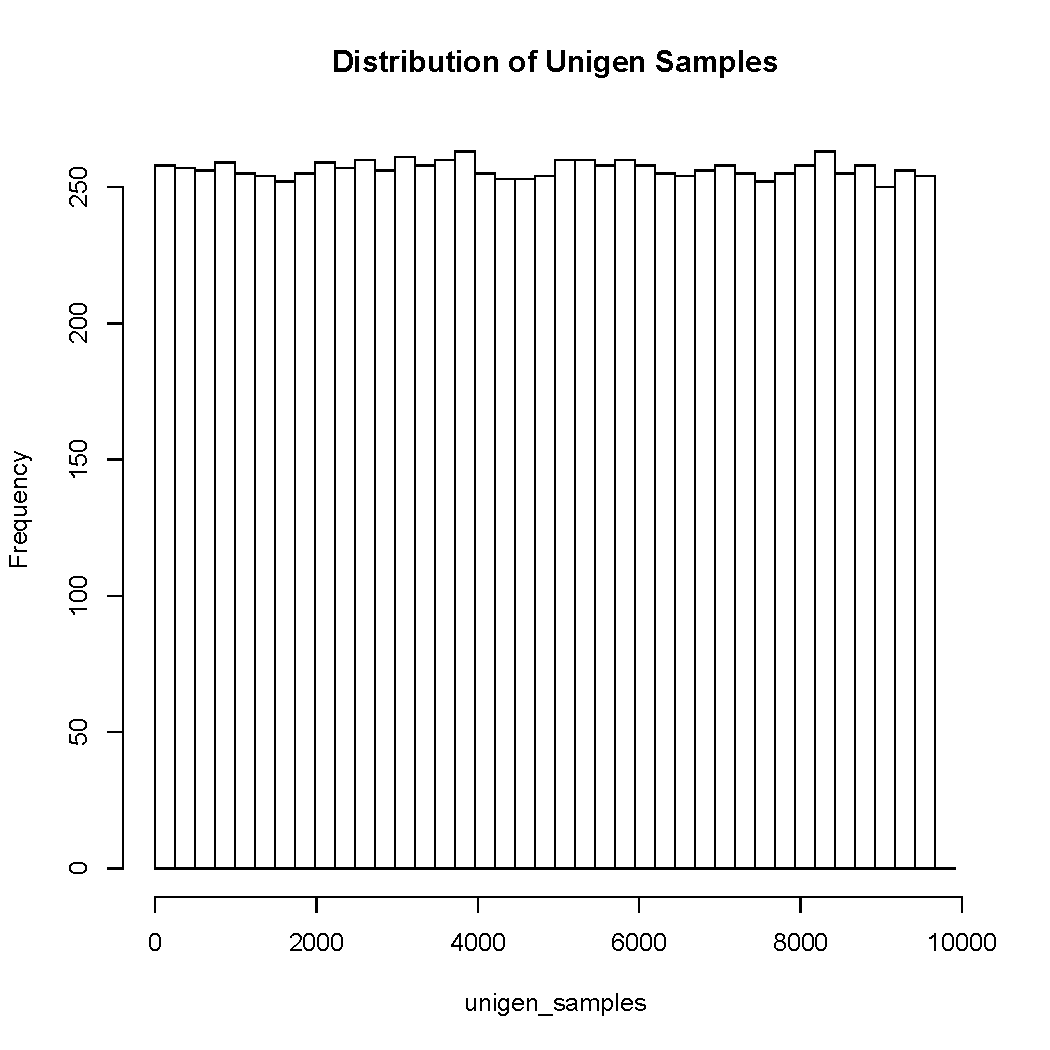
\includegraphics[origin=c,width=12cm]{../figures/unigen-samples.pdf}}
\caption{Distribution of Sequences Sampled by Unigen}
\label{fig:unigen_samples}
\end{figure}


\subsection{KUS}

% time python /home/drautb/GitHub/meelgroup/KUS/KUS.py --dDNNF d-DNNFs/stroop-3.dnnf --samples 10000 --outputfile d-DNNFs/stroop-3-kus-10000-samples.out
% ('Time taken to parse the nnf text:', 1.0481359958648682)
% ('Time taken for Model Counting:', 1.0421910285949707)
% ('Model Count:', 112409849997702614628L)
% ('Time taken by sampling:', 16.441092014312744)
% ('Samples saved to', 'd-DNNFs/stroop-3-kus-10000-samples.out')
% python /home/drautb/GitHub/meelgroup/KUS/KUS.py --dDNNF d-DNNFs/stroop-3.dnnf  25.76s user 0.59s system 102% cpu 25.828 total

KUS sampled 10,000 trials sequences, all of which were unique.

\begin{figure}
\centering
\centerline{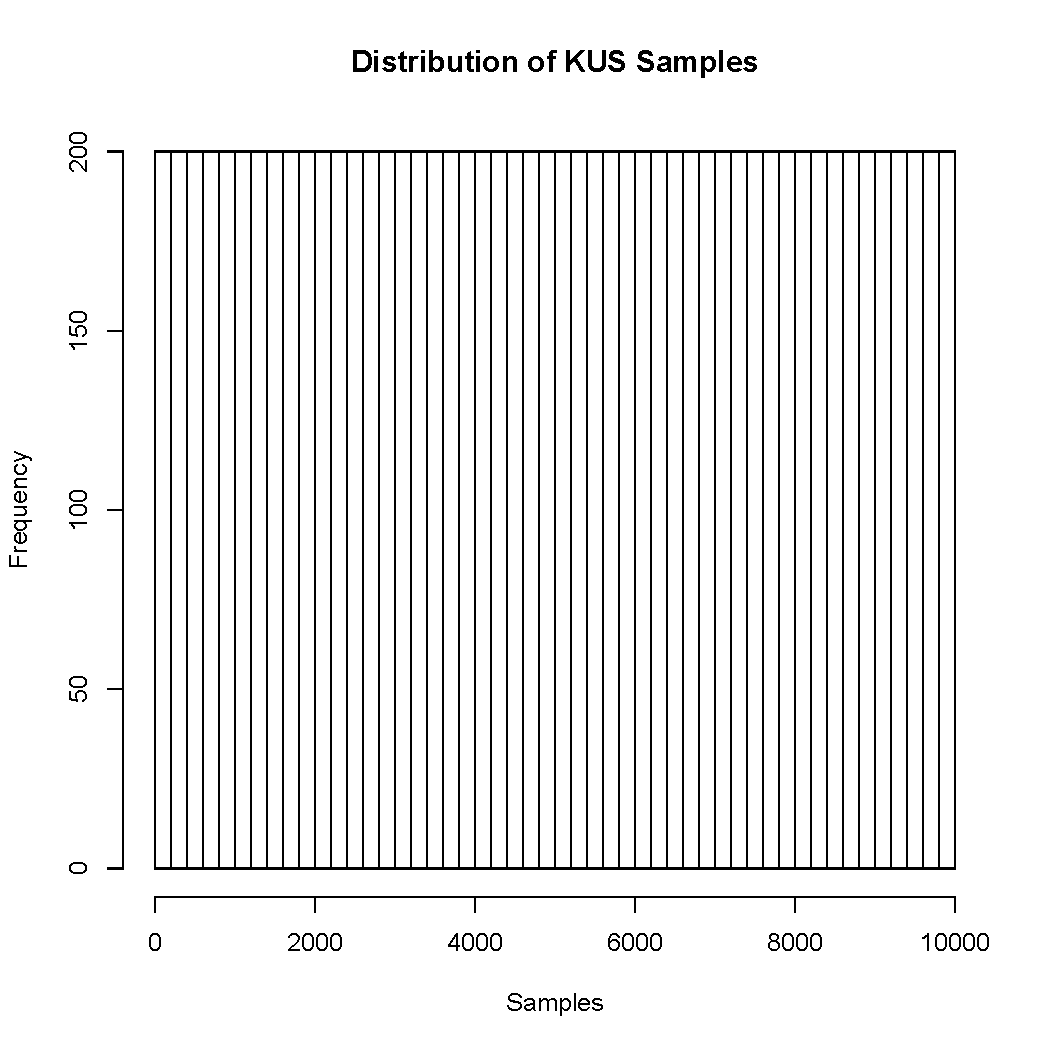
\includegraphics[origin=c,width=12cm]{../figures/kus-samples.pdf}}
\caption{Distribution of Sequences Sampled by KUS}
\label{fig:kus_samples}
\end{figure}


\subsection{Spur}

% time /home/drautb/GitHub/ZaydH/spur/build/Release/spur -q -s 10000 -cnf stroop-3.cnf -out stroop-3-spur-10000-samples.out
% /home/drautb/GitHub/ZaydH/spur/build/Release/spur -q -s 10000 -cnf  -out   30.97s user 0.23s system 99% cpu 31.250 total

Spur sampled 10,000 trial sequences, 9,664 of which were unique. 332 sequences were selected twice, and 2 were selected three times. No sequences were selected more than three times.

\begin{figure}
\centering
\centerline{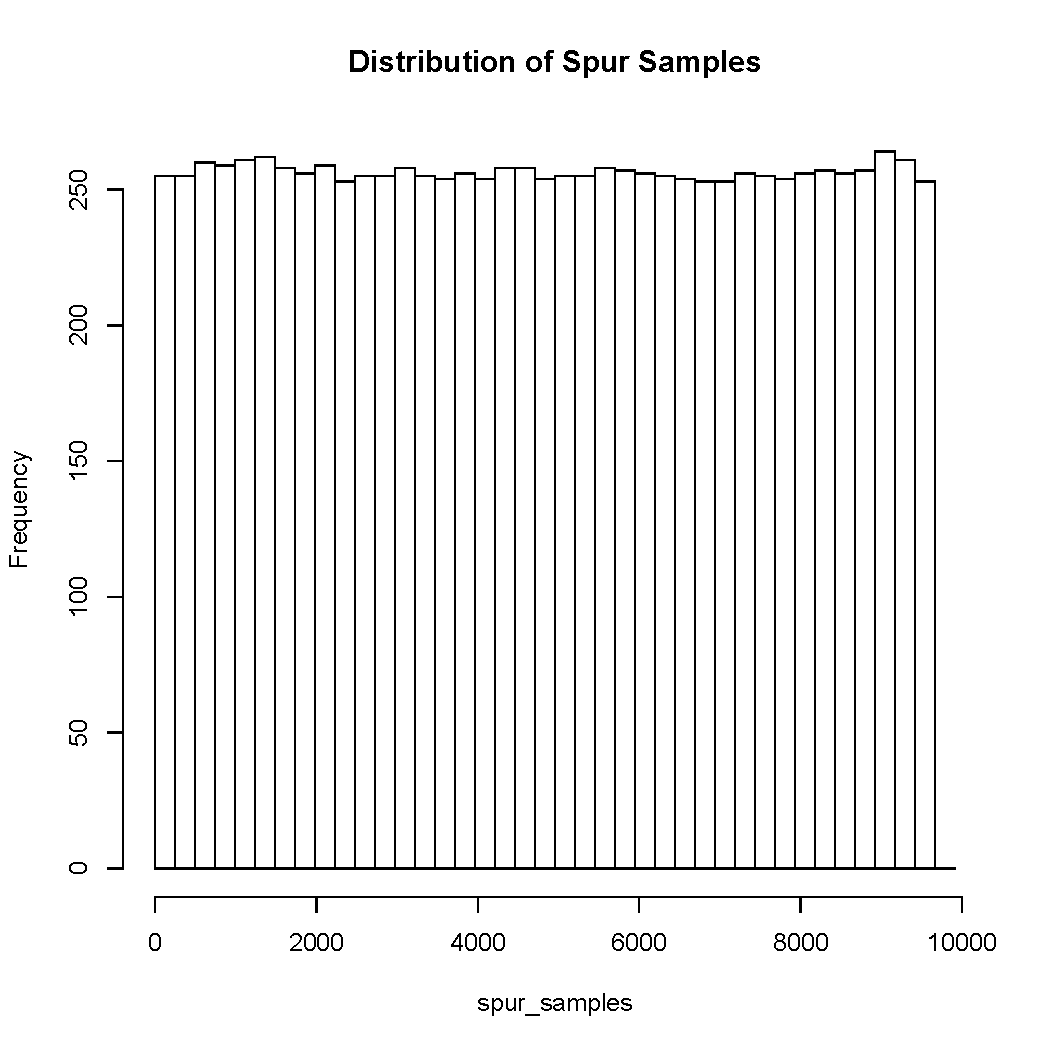
\includegraphics[origin=c,width=12cm]{../figures/spur-samples.pdf}}
\caption{Distribution of Sequences Sampled by Spur}
\label{fig:spur_samples}
\end{figure}


\subsection{CryptoMiniSat}

In contrast to the previous tests, when a SAT solver is used to generate individual samples incrementally by adding negated solutions to the prior formula, the same samples are generated each time. We used CryptoMiniSat to generate 10,000 samples as well, in groups of 100. Exactly the same set of 100 samples was generated each time.


\section{Summary}

None of the current tools for sampling SAT formulae are capable of handling the scale of practical experimental designs. Although the number of variables and clauses in the CNF for these experiments is reasonable, the factorial explosion in the number of solutions to the formulae overwhelmed each tool that we tested.





